\documentclass[10pt]{report}
\usepackage{fullpage}
\usepackage{graphicx}
\usepackage{verbatim}
\usepackage{subfig}

\newcommand{\HRule}{\rule{\linewidth}{0.5mm}}

\begin{document}
\begin{titlepage}
\begin{center}
% Upper part of the page

\includegraphics[width=0.15\textwidth]{logo.jpg}\\[2cm]    
\textsc{\LARGE CS 680}\\[1.5cm]

\textsc{\Large Computer Graphics}\\[0.5cm]


% Title
\HRule \\[0.4cm]
{ \huge \bfseries Air Hockey User and Technical Manual}\\[0.4cm]

\HRule \\[1.5cm]

% Author and supervisor
\begin{minipage}{0.4\textwidth}
\begin{center} \large
\emph{Author:}\\
Joshua \textsc{Gleason}
Marvin \textsc{Smith}
\end{center}
\end{minipage}
\vfill
% Bottom of the page
{\large \today}
\end{center}
\end{titlepage}
\newpage

%**************************************************%
%                    INTRODUCTION                  %
%**************************************************%
\section*{Air Hockey Overview}


\section*{Opinions}


\section*{Time Spent}



\section*{Extra Credit}
\begin{description}
\item[High Scores Window] accessible from either the menu or by pressing '8' key
\end{description}

%**************************************************%
%                    USER MANUAL                   %
%**************************************************%
\clearpage
\section*{User Manual}
\subsection*{Introduction}
This manual will introduce you to the basic functions of the AirHockey 
game. Figure \ref{fig:game} shows the basic layout of the game.

\begin{figure}[!h]
\centering
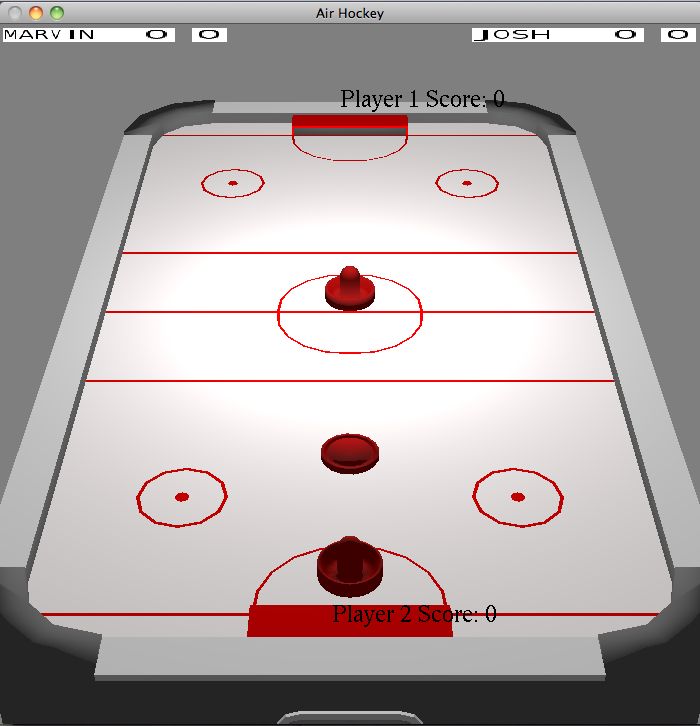
\includegraphics[width=3in]{game.png}
\caption{Basic Layout of Air Hockey}
\label{fig:game}
\end{figure}

\subsection*{Navigation}
There are many different features in Air Hockey. To get to all of them, you will
need either the keyboard or the menu. To access the menu, click on the screen with
the right-mouse button. Figure \ref{fig:menu} shows the basic layout of the menu. 

\begin{figure}[!h]
\centering
\subfloat[Main Menu]{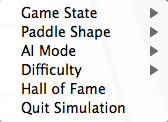
\includegraphics[width=1.3in]{menu.png}}
\subfloat[State Submenu]{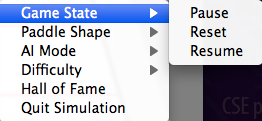
\includegraphics[width=1.8in]{menu_state.png}}
\subfloat[Shape Submenu]{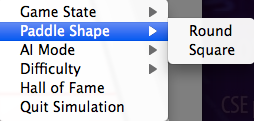
\includegraphics[width=1.7in]{menu_shape.png}}\\
\subfloat[AI Submenu]{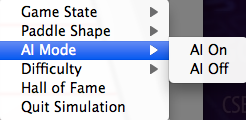
\includegraphics[width=1.6in]{menu_ai.png}}
\subfloat[Difficulty Submenu]{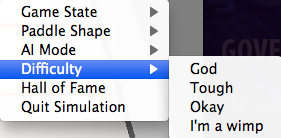
\includegraphics[width=1.7in]{menu_difficulty.png}}
\caption{Basic Menu Layout of Air Hockey}
\label{fig:menu}
\end{figure}

\clearpage
\section*{Technical Manual}
\subsection*{Design Decisions}

\begin{description}
\item[something]
\end{description}

\subsection*{Deficiencies}

\subsection*{Areas for Improvement}

\end{document}
